\documentclass[conference]{IEEEtran}
\usepackage[utf8]{inputenc}
\usepackage{amssymb}
\usepackage{graphicx}
\usepackage{pifont}
\usepackage{multirow}
\usepackage{url}
\newcommand{\cmark}{\ding{51}}%

\title{Aduno: Real-Time Collaborative Work Design In A Shared Workspace}
%\author{\IEEEauthorblockN{Braden Simpson}
%\IEEEauthorblockA{University of Victoria\\
%Victoria, British Columbia\\
%braden@uvic.ca}
%\and
%\IEEEauthorblockN{Eirini Kalliamvakou}
%\IEEEauthorblockA{University of Victoria\\
%Victoria, British Columbia\\
%ikaliam@uvic.ca}
%\and
%\IEEEauthorblockN{Nathan Lambert}
%\IEEEauthorblockA{University of Victoria\\
%Victoria, British Columbia\\
%nlambert@uvic.ca}
%\and
%\IEEEauthorblockN{Daniela Damian}
%\IEEEauthorblockA{University of Victoria\\
%Victoria, British Columbia\\
%danielad@cs.uvic.ca}}

\author{\IEEEauthorblockN{Braden Simpson\IEEEauthorrefmark{0}, Eirini Kalliamvakou\IEEEauthorrefmark{0}, Nathan Lambert\IEEEauthorrefmark{0} and Daniela Damian\IEEEauthorrefmark{0}}
\IEEEauthorblockA{\IEEEauthorrefmark{0}Department of Computer Science, University of Victoria\\
brsmp@acm.org, ikaliam@uvic.ca, nlambert@uvic.ca, danielad@cs.uvic.ca}}

\begin{document}
\maketitle

\begin{abstract}
In this paper we introduce Aduno, a shared workspace tool that allows distributed software teams to collaboratively establish and prioritize work items for the purposes of task management and planning during the design phase. Aduno is highly visual and real-time, offering features that are often lacking from other popular collaborative development tools. In line with the growing adoption of Github, Aduno also links to Github's issue tracker and easily translates work items on a whiteboard to project work items. Here, we describe the concept and design of Aduno and present its initial evaluation.
\end{abstract}

\section{Introduction \& Motivation}
\label{sec:intro}

%As teams today become more distributed, they need tools that support their collaboration and keep members aware of each others' actions, to minimize disruptions in their workflow and coordination. Distributed teams need to collaboratively negotiate and carry out work tasks, so tools that combine real-time editing with visual workspaces help towards commonly agreed-upon task management. 

As software development has become highly distributed, teams need to coordinate for different sets of activities until they have built the end product. This creates a need for tools that support their collaboration and keep members aware of each others' actions, to minimize disruptions in their workflow and coordination. During the earlier stages of development, developers need to establish work items to plan and organize their work around. A comparison between some of the most popular and widely used tools for collaborative software development (Table~\ref{tab:otherservices}), shows that they mostly rely on text-based methods of establishing work items and handling workflow, not providing highly visualized features and not being particularly real-time. 

%Aduno aims to extend the functionality provided by these tools by addressing this limitation.

\begin{table}[h]
\begin{center}
\begin{tabular}{@{\hspace{.2cm}}ccc@{\hspace{.2cm}}c@{\hspace{.2cm}}c@{\hspace{.2cm}}c@{\hspace{.2cm}}c@{\hspace{.2cm}}}
\hline
Similar Services&  Real-time&   Control of&  Tags&    Visual layout&      Chat&\\
 & & WorkItems& & & &\\
\hline
Github Issues   &	-&	        \cmark&	                \cmark& -&                  -\\ 
Google Code     &   -&          \cmark&                 -&      -&                  -\\
Jazz            &   -&          \cmark&                 \cmark& -&             -    \\
MindMeister & \cmark& -& -& \cmark& - \\
Trello & \cmark& -& \cmark& -& \cmark\\
Aduno           &   \cmark&     \cmark&                 \cmark& \cmark&             \cmark\\
\hline
\end{tabular}
\end{center}
\caption{Comparing Collaborative Tools\label{tab:services}}
\label{tab:otherservices}
\end{table}

The limited visualization and real-time editing in these collaborative software development tools might still be efficient for teams that have also more informal means of communicating and negotiating work, but distributed teams mostly miss out on these direct communication methods. We hypothesize that \textit{a highly visual, real-time environment for creating and managing work items between team members, can better support developers through the design process and can produce benefits in terms of the clarification, errors and speed} of this part of the work process. 

We introduce Aduno, a shared workspace application that enables visually creating and organizing work tasks in real time, targeted towards software development teams. Our solution originates from the basic concept of a shared whiteboard, incorporates communication and collaborative features that are present in the state-of-the-art tools developed for the same target group, and successfully supports group and workspace awareness as a collaborative basis in development projects. In line with the growing best practice of using Github as a collaborative platform for development management, Aduno supports synchronizing with Github's issue tracker for quickly translating work items to actionable pieces of development effort.  Aduno uses the real time collaborative aspects of whiteboards, and extends it to more distributed settings, while leveraging a persistent data source like Github.

Aduno has been evaluated by means of an expert judgement study involving eight users. The aim of this initial evaluation was to test the usability of the tool for distributed collaboration between software developers, and rank how well it supports collaborative behaviour. The experts have provided positive feedback and the results indicate that Aduno successfully fits the intended purpose.  The future plans for Aduno include an extended quantitative evaluation study, to investigate how it can support distributed software development teams effectively with task management during the design phase.

%The paper is structured as follows: We present background and work relating to building groupware applications supporting collaborative work in Section~\ref{sec:background} and explain how we used this as a foundation for Aduno's requirements. We then present the tool's concept, functionality, and design decisions in Section~\ref{sec:concept} and provide three scenarios of use as examples in Section~\ref{sec:scenarios}. We describe the initial evaluation we carried out with a team of experts in Section~\ref{sec:evaluation} and Section~\ref{sec:results} presents the evaluation results. We describe our future work goals in Section~\ref{sec:future} and conclude the paper in Section~\ref{sec:conclusion}.


\section{Background \& Related work}
\label{sec:background}

Requirements for building Aduno were systematically derived from the background knowledge on {\sc cscw} applications and the features that successful groupware should provide. 

In building groupware applications, effort has been placed on how to support grounding in collaboration through visibility and co-presence. McCarthy et al. \cite{MCMM91} conducted experiments with teams collaboratively solving problems both with and without a shared space and found that the degree of disagreement was inversely related to the development of common ground within teams. Gutwin et al. \cite{GRG96} enhanced a shared workspace application with widgets providing activity and location information of participants and found that the add-ons provided value towards the successful completion of the tasks and the degree of awareness maintained within the team.

\begin{table*}
  \centering
  \begin{small}
    \begin{tabular}{p{9em}lcc}
      \hline
      \textbf{Category} & \textbf{Element} & \textbf{Questions} \\
      \hline
      \multirow{3}{9em}{\textbf{Who}} & Presence & Is anyone in the workspace? \\
      & Identity & Who is participating? Who is that?  \\
      & Authorship & Who is doing that? \\
      \hline
      \multirow{3}{9em}{\textbf{What}} & Action & What are they doing? \\
      & Intention & What goal is that action part of? \\ 
      & Artifact & What object are they working on? \\
      \hline
      \multirow{4}{9em}
      {\textbf{Where}} & Location & Where are they working? \\
      & Gaze & Where are they looking? \\
      & View & Where can they see? \\
      & Reach & Where can they reach? \\
      \hline
    \end{tabular}
  \end{small}
  \caption{Elements of workspace awareness from \cite{GG02}}
  \label{tab:Gutwin}

\end{table*}


Gutwin \& Greenberg \cite{GG02} produced a conceptual framework of the information required for workspace awareness (Table~\ref{tab:Gutwin}) with the basic elements coming from answering the questions of ``who, what and where''. These elements make up workspace awareness and although in a physical setting they are easy to attain, they need to be explicitly supported in groupware applications. Designers of collaborative tools need to account for workspace awareness through the features they offer and help a collaborating team establish and maintain common ground to ensure a successful result.
%CITE
Tools that support web-based collaborative work that is real-time are a definite trend today, enabling teams to achieve common ground faster, maintain awareness of others' actions more effectively, and coordinate more smoothly. Google Docs, a web-based text, spreadsheet, presentation and form editor whose data storage is provided by Google is only one successful example. Google Docs~\cite{SIRM07} is a truly collaborative tool for document editing, allowing sharing and editing by multiple users at the same time. The design features offered by Google Docs are awareness solutions that allow collaborators to have real-time information other users' activity and location in the form of remote cursors, participant lists, revision history, etc.

Distributed software development teams face the same challenges of distributed collaboration in terms of grounding and maintaining workspace awareness. Especially during the initial stages of a software development project, effort is required to define and prioritize work items as well as assign or negotiate who is responsible for what. As distributed teams aim towards leaner organizational structures and modularized work items to overcome some of the challenges of distribution \cite{Herbsleb07, HG99, Parnas72}, tools that enable teams to define work items collaboratively, as a starting point for their development work, are essential. The underlying rationale here is that the modularity of the product design will decide the modularity of the work tasks and if this process can be as transparent and as commonly agreed upon as possible in the project, it will set the stage for smoother coordination down the road. 

%This rationale is also in line with Conway's Law \cite{Conway68} which is as relevant to distributed software teams today as ever.

Based on this background knowledge, the design of Aduno is aimed towards supporting distributed teams during the design phase when work item creation and management are crucial. Our goal is to implement features that visually provide workspace awareness to team members, and embed them on a web-based infrastructure to allow for real-time collaboration. Aduno also promotes a more flat and flexible team structure, allowing team members to negotiate and establish roles through self-organization by working on specific work items, or outside the tool.


%\subsection{{\sc cscw} application success and failure}
%Grudin \cite{Grudin88} discussed the main reasons behind the failure of {\sc cscw} applications. Through reviewing cases of {\sc cscw} application areas that have fallen short of expectations, he concluded that there are three factors that can lead {\sc cscw} applications to not be adopted. Below, we summarize his insights and highlight how these created the initial requirements for Aduno.
%
%\textbf{Disparity between effort and benefit.} Using automatic scheduling applications as an example, Grudin identified that the application's use was not mutually beneficial to the groups involved, and this negatively affected adoption. An automatic scheduler for meetings was beneficial to the time-conscious manager that initiated meetings, but only required extra effort on behalf of group members that were positioned lower in the organizational hierarchy. The latter group wouldn't have ordinarily kept up with automatic schedulers, but were now required to do so to provide benefit to the regular user group of this application. Grudin's view was that the underlying cause of the problem was the erroneous analogy of the single-user application model used for groupware.
%
%This kind of mismatch created a fundamental initial requirement for Aduno. As a tool intended to support groups, it is designed to be used by the entire group and \textit{provide mutual benefit}. Identifying, creating, and linking tasks in a real-time manner that makes the whole group aware of the process, while leaving room for task negotiation since it is done collaboratively, brings benefit to all users involved in the software development project, from the project manager to the developer.
%
%\textbf{Difficulty of {\sc cscw} application evaluation.} Aduno is by design aimed towards group use, and disregards group hierarchy or roles inside the tool.  Dourish et al. found that having dynamic role creation in the collaborative application was a positive factor~\cite{Dourish:1992:ACS:143457.143468}, and this was an aspect that was incorporated into Aduno. Grudin's view of evaluating {\sc cscw} applications was that it is more complex because it involves multiple users and different groups. He proposed drawing on social science techniques to help with identifying group dynamics and trying to incorporate this into the evaluation. Aduno, having disposed of hierarchical roles inside the tool, creates \textit{less demands for using specialized techniques}. Aduno's evaluation was done through an expert study where its usability and fit for the intended users was verified.

\section{Aduno: Features and Design}
\label{sec:concept}

%\subsection{Framework describing workspace awareness}
%The next background element that impacted Aduno's functional requirements is 
%Aduno is an interface that uses real time and visual elements to assist developers and others when creating and editing work items.  Many collaborative development environments (Table~\ref{tab:otherservices}) provide an almost exclusively asynchronous approach to developing articulative work, and this is one of the motivators for Aduno, which poses to extend these environments by enabling synchronous collaborative experience. Github was chosen as the preferred backend because of its robust and open API, in addition to it hosting almost three million open-source repositories. 

%The main aspects of collaborative applications that were the basis of the architectural design decisions of Aduno are \emph{speed}, \emph{synchronicity}, and \emph{simplicity}.  With these components in mind, the development team built Aduno to be able to interface with the Github API, or other RESTful services, to provide a faster, more effective way to collaborate on articulative tasks.  

%\subsection{Aduno's functionality}
Aduno offers a shared workspace where a software development team with a Github-hosted project, can collaboratively manipulate their workflow using visual components. Teams can sign in with their Github account details and access their repositories, and Aduno imports the project's issues on the workspace in the form of work items. Users can create, edit, link, and move around work items to organize their joint actions, and coordinate about them by communicating through the tool's chat area. In real time users can also see all changes that other team members are making on the work board and Aduno's visual layout allows them to maintain workspace awareness. The contents of the work board can then be exported to Github's issue tracker, integrated directly into the team's workflow.

The functionality offered by Aduno is mostly targeted towards the initial stages of a software project's life cycle, when task management activities are more intense. During the software design phase a team needs to commonly agree on work structure. Identifying, creating, and linking tasks in a real-time manner that makes the whole group aware of the process, while leaving room for task negotiation since it is done collaboratively, brings benefit to all users involved in the software development project, from the project manager to the developer. Once work items are in the project's issue tracker then the team can smoothly begin their coding tasks.

Aduno proposes enhancements on two levels of collaborative work design for software development; creating a \textit{real-time} collaborative environment and making use of a \textit{highly visual interface}. Aduno offers the following four areas of functionality:

\begin{itemize}
	\item \textbf{Team communication and coordination}
	\item \textbf{Synchronization to Github's issue tracker}
	\item \textbf{Workflow management}
	\item \textbf{Organization of work items on a work board}
\end{itemize}

%Below we present how each functionality area is supported through Aduno as well as how the tool's features promote workspace awareness as per Table~\ref{tab:Gutwin}. 
%\subsection{Feature description}
%
%\textit{Team communication and coordination} is an integral part of the software development process and is a challenge whenever collaborating teams are distributed. Although it is typical for project management systems in services such as Github to allow comments on each issue, we have included a chat area in Aduno. The comments on work items in Github are used for asynchronous communication, and this was not sufficient for our tool. A chat system provides users with a secondary communication channel that allows them to engage in a synchronous discussion about work items that would not typically be appropriate for asynchronous work item comments. Since comments in Github must also be attached to only one work item, having this chat area helps teams develop broader goals and facilitates common ground through more in-depth conversation.
%
%\textit{Persistent project data synchronization} is an important and highly functional aspect of Aduno.  The data modelled in Aduno is transferred as you work to issue trackers such as Github, meaning teams are able to enjoy the best of both worlds by using Aduno's highly visual, real-time environment for design tasks, and smoothly integrating with their existing workflow. Once a user signs in Aduno with their Github credentials they have all their repositories and respective issues in place and they can select what they want to work on. When an edit is performed on a work item in Aduno, the ``Sync" indicator at the top right of the item turns from green to orange to signal that there is an unsynchronized change. To synchronize with Github, the user can click on the ``Sync All" button at the top of the page, or they may click on a work item's ``Sync" button to synchronize it individually. This gives the team more control over what work items get synced with the associated service.
%
%\begin{figure*}[t]
%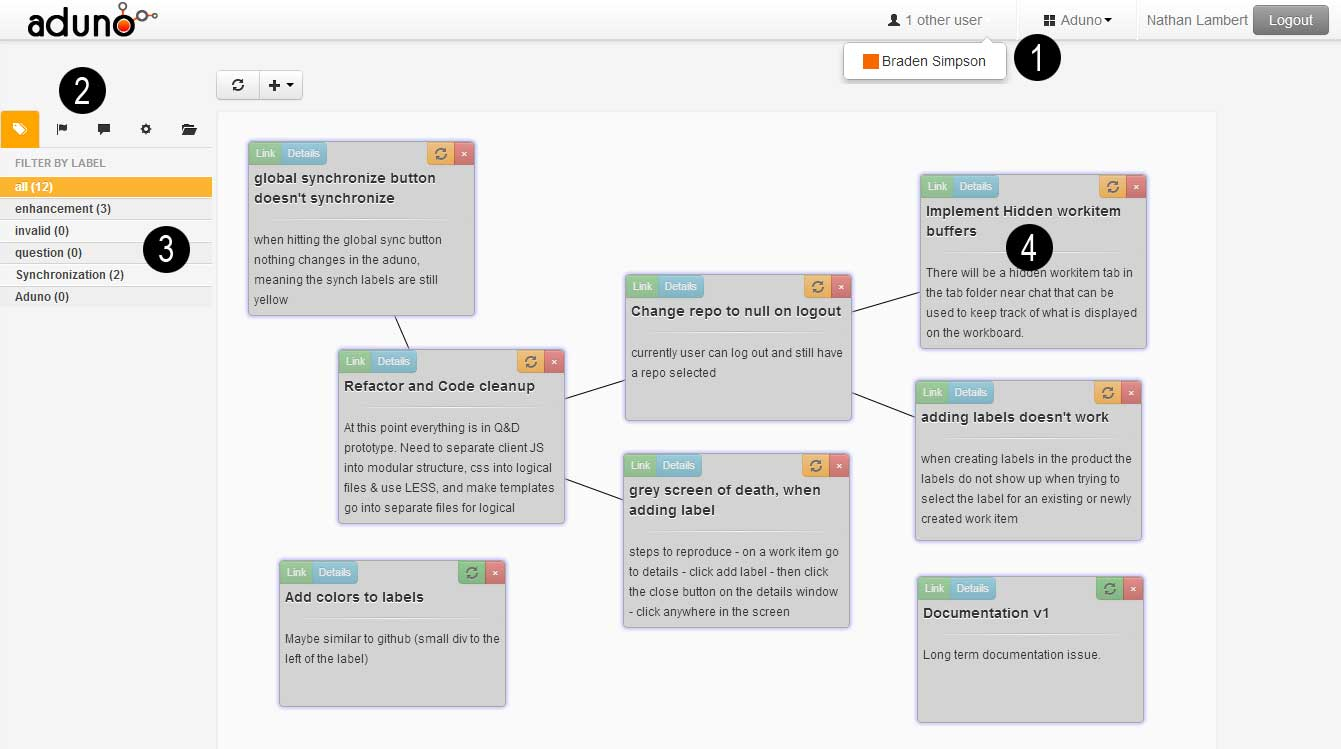
\includegraphics[width=\textwidth]{aduno-screenshot}
%\caption{Aduno Screenshot}
%\label{fig:adunoscreenshot}
%\end{figure*}
%
%
%Figure~\ref{fig:adunoscreenshot} shows a typical example of Aduno's interface, with a few emphasized features, described as follows: 
%\begin{enumerate}
%	\item \textbf{Navigation} - All global controls shown on this bar including options to authenticate, change repository, change user settings, and see other online users.
%	\item \textbf{Workflow} - A tabbed container allows the user to switch between the different features, such as label filtering, milestones, chat, and repository settings.  
%	\item \textbf{Labels} - Labels are optional tags that are a method for filtering and categorizing work items.  They offer a good way for users to be able to quickly switch between different areas of the project.  
%	\item \textbf{Work Items} - These are the building blocks of Aduno. They are representations of the issues in Github, except they can be dragged around the work board (the large whiteboard-like area that holds the work items), edited in real time, linked to each other, and modified in any way a Github issue could be. 
%\end{enumerate}
%
%A major functionality proposed by Aduno is the ability to \textit{organize work items on the work board}. Users can create, edit, link, and move work items on the work board, and their changes are transparent to all collaborators. The feature to link work items is particularly important, as in other services work items are displayed in a list without any notion of priority. Although they allow for links between work items, users must follow a link to view them. Having a visual representation of the links allows users to quickly glance at the related work items. Allowing users to move the work items around on the work board gives them several opportunities, including being able to arrange them in whatever context is appropriate and order them accordingly. Work items can also be grouped together to imply a connection.  In Figure~\ref{fig:adunoscreenshot}, the visual representation of links can be seen, which gives the work items more context, and allows for richer visual models.  
%
%\subsection{Maintaining workspace awareness}
%
%Gutwin's \& Greenberg's \cite{GG02} framework of information to support workspace awareness for real-time groupware is intended to aid the design of real-time groupware and makes use of different theories and observational studies. The framework is especially relevant to Aduno's design as it targets real-time distributed groupware, shared workspaces and both generational and execution tasks. In terms of group size, the framework mainly discusses small groups. For the current design state of Aduno this fits the tool's purpose, although one of the future goals for Aduno is to investigate how it scales in order to be used by larger groups.
%
%Referring back to Table~\ref{tab:Gutwin}, awareness relating to the ``Who'' category sets the aim for groupware to provide information of others present in the workspace and who they are, while authorship information maps an action to the person performing it. Regarding the ``What'' category, a tool must successfully communicate information about what other users are working on, either in detail or in general. Aduno's features, as discussed below, cover these two categories, fulfilling the requirements for real-time groupware supporting awareness. Information relating to the ``Where'' category, is intended for large workspaces and better fitted to construction tasks, such as the one discussed in \cite{GRG96}. To this end, they are not explicitly part of Aduno's design. However, location and gaze information can be inferred by the work items a user is moving around the workspace.
%
%The elements of workspace awareness outlined in Table~\ref{tab:Gutwin} should be completely fulfilled in an effective collaborative application, although some of them are not applicable to this tool. As previously mentioned, awareness of gaze, view, and reach would add much complexity to the tool without providing much benefit. However, the remaining elements play an important role in user awareness with Aduno.
%  
%{\bf Presence} – An indicator in the navigation bar at the top of the screen signals the presence of other users.  Also, whenever users are interacting with controls in the workspace, they have their presence made known in the form of their unique color and username badge shown.
%
%\begin{figure}[htb]
%\centering
%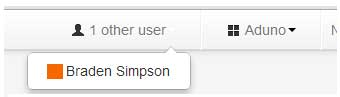
\includegraphics[scale=0.5]{aduno01}
%\caption{Online user indicator}
%\label{fig:otherusers}
%\end{figure}
%
%{\bf Identity} – Clicking on the indicator shows a dropdown listing of all the current online users. A color unique to that user is displayed next to their name.  This is a globally used identity that is persistent to all items related to the user. 
%
%{\bf Authorship} – When a user is editing a work item, their name is displayed at the bottom of it to indicate that they are currently working on it.
%
%\begin{figure}[htb]
%\centering
%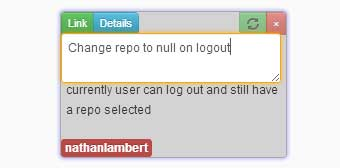
\includegraphics[scale=0.5]{aduno02}
%\caption{Work Item Being Edited}
%\label{fig:workitem}
%\end{figure}
%
%{\bf Action} – Editing actions result in real-time data propagation, immediately showing changes across all clients that are connected to the same repository.  
%
%{\bf Intention} – The intention of most work item edits would likely be apparent as the edits are being done. When a user clicks and holds, this reveals their intention to move an item, while clicking and releasing reveals an intention to edit it. Broader goals may be discussed in the chat window. Chat commands are used to provide contextual awareness to the users.  For example, someone can reference a work item by using it's ID in the chat window.
% 
%{\bf Artifact} – As shown in Figure~\ref{fig:workitem}, usernames are displayed at the bottom of it to indicate who is currently working on an item.
%
%{\bf Location} – The location of the user’s work is shown by the username attached to a work item when they are doing edits. If the user moves a work item around, their location becomes apparent.
%
%{\bf Ownership} - Storing a history of modifications to work items is a way to add awareness for users that are not synchronously working, and allows for reflection on the creation process.
%
%%A summary of Aduno's functionality is presented in Table~\ref{tab:summary}.
%%
%%\begin{table*}
%%  \centering
%%  \begin{small}
%%    \begin{tabular}{ccc}
%%      \hline
%%      \textbf{Functionality} & \textbf{Features} & \textbf{Workspace Awareness} \\
%%      \hline
%%      \multirow{2}{9em}{\textbf{Communication/ Coordination}} & User indicator & Presence - Identity \\
%%      & Chat & -  \\
%%      \hline
%%      \multirow{2}{9em}{\textbf{Github import/export}} & Select repositories & - \\
%%      & Sync indicator & - \\ 
%%      \hline
%%      \multirow{2}{9em}
%%      {\textbf{Workflow management}} & Tabs & - \\
%%      & Label filters & - \\
%%      \hline
%%      \multirow{5}{9em}
%%      {\textbf{Work item organization}} & Create work items & Action \\
%%      & Edit work items & Action-Intention \\
%%      & Link work items & Action \\
%%      & Username display & Authorship-Artifact-Location \\
%%      & Move work items & Intention-Location \\
%%      \hline 
%%    \end{tabular}
%%  \end{small}
%%  \caption{Summary of Aduno's functionality}
%%  \label{tab:summary}
%%
%%\end{table*}
%
%
%%\subsection{Purpose}
%%Aduno was constructed around the requirements described in Section~\ref{sec:background}.  From this model, the requirements were gathered and formulated into implementation.  
%
%\subsection{Architectural design}
%With \emph{speed} being one of the most important aspects of the design, the architecture chosen for the server-side technology is crucial.  Node.js\footnote{A platform for building fast, scalable network applications, http://nodejs.org}, a platform of server-side JavaScript built on Google Chrome's V8 JavaScript runtime, was chosen as our platform.  Node has been quickly adopted as a powerful platform for web applications such as Cloud9\footnote{A collaborative web IDE built in Node.js}, LinkedIn, Windows Azure and more.  Tilkov \& Vinoski~\cite{TV10} have shown Node as a viable choice for non-blocking web applications.  Using Node allows Aduno to be deployed easily to the Amazon Elastic Cloud compute instances as a cloud service, as well as simple setup for private instances.
%
%\emph{Synchronicity} is a crucial component of Aduno and was a great influence over the frameworks chosen for the tool.  The Meteor Framework\footnote{An open-source web application framework focused on real-time updates} was chosen to support asynchronous data among users, since Meteor pushes changes out to clients dynamically, updating their screens without refreshing, and unobtrusively keeping users synchronized.  
%
%\emph{Simplicity} is a key point in any application that needs to attract its new users, and Aduno had this principle as a top priority.  The web toolkit used to support this is Twitter Bootstrap, a very common open-source user interface toolkit, with approximately 100 developers.
%
%\section{Scenarios of use}
%\label{sec:scenarios}
%In this section we describe three typical example scenarios for Aduno, most useful for developers in distributed teams. The scenarios include a team collaboratively creating work items, and single users filtering system areas and examining relationships between tasks.
%
%\subsection{Collaboratively Creating Work Items}
%To do preliminary design of a new feature on a large web application, a team of developers and managers must meet to construct the work items for the feature.  
%\begin{enumerate}
%	\item All members have a distributed meeting, sign into Aduno, and load the appropriate repository.
%	\item Members are able to chat, to start the meeting.  
%	\item Members create work items with initial requirements, high level and unrefined.
%	\item Members edit work items and transparently collaborate with others in real time, catching mistakes and asking clarification questions as they appear.  The work items show the currently editing user, and updates across all clients. 
%	\item Labels and assignees are added as the work items become more well-defined, as the areas of the feature become more concrete.
%	\item Synchronization with the company repository has integrated the new work into the respective developers workflows, and work can begin.
%\end{enumerate}
%
%\subsection{Visually Representing System Areas}
%A single user wants to view all work items related to a specific system area, \textit{performance}, for example. 
%\begin{enumerate}
%	\item User logs in and selects the repository.
%	\item User selects the \textit{performance} label in the labels panel.
%	\item The system clears the work board and displays all work items that have the \textit{performance} label.  All of the links between work items are displayed visually with lines connecting the work items.
%	\item The user may rearrange and interact with the work items, as well as see any other users that are online.
%\end{enumerate}
%
%\subsection{Examining Relationships Between Tasks}
%A single user wants to view and interact with a work item and its related tasks. 
%\begin{enumerate}
%	\item User logs in and selects the repository.
%	\item The user views a work item and all of the interrelated ones by following the links associated with the respective work item.
%	\item The system shows all the users that are currently working on these work items.
%\end{enumerate}

\section{Evaluation \& Results}
\label{sec:evaluation}

To evaluate Aduno's usability and fit for the intended use, we carried out an expert judgement study involving eight users, forming four pairs. The participants had on average four years of experience in distributed software development and have participated in multiple collaborative projects.


%The participants were graduate and undergraduate students in a {\sc cscw} course who have been introduced to {\sc cscw} issues in the design and evaluation of groupware. 
\subsection{Setup}
The experts were invited to participate in the evaluation session and, after indicating their availability, were randomly assigned to pairs. In each evaluation session, the experts were first given a short demonstration of the tool's features and the shared workspace layout. Following that, participants were given a short description and high-level requirements for a fictional website they would have to build in collaboration with their partner. They were asked to use the tool to collaboratively define and link work items. The experts were not allowed to communicate outside the tool, as a way to account for them being distributed. For the final part of the evaluation session, experts were given a short questionnaire to fill out, evaluating the tool's fulfillment of its purpose as well as its potential impact on a project.

\subsection{Questionnaire}
The questionnaire's design was guided by insights from the literature regarding collaborative behaviours that should be successfully supported by {\sc cscw} applications. Clark \cite{Clark96} defined the following eight behaviors for collaboratively carrying out joint actions:

\begin{itemize}
\item \textbf{Connection} -- locating with whom to collaborate and how to contact them
\item \textbf{Transmission} -- sending a message
\item \textbf{Notification} -- alerting the intended party of an incoming transmission
\item \textbf{Identification} -- designating the sender, receiver, and subject of a transmission
\item \textbf{Common Ground Preservation} -- establishing and maintaining a shared context and meanings in transmissions
\item \textbf{Confirmation} -- notifying the sender of a transmission that it has been received
\item \textbf{Synchronization} -- orchestrating actions to facilitate joint action
\item \textbf{Election} -- group process of selecting among alternatives
\end{itemize}

Thompson \cite{Thompson67} defined three types of coordination, \textit{standardized}, \textit{planned} and \textit{mutual adjustment}. Software development fits under the latter type of coordination, which includes all collaboration behaviors. As a result, tools such as Aduno, aimed towards supporting this kind of tasks, must include features that cover the respective behaviors. To account for this during the evaluation, the questionnaire was designed to check how well these behaviours were supported. The questionnaire used can be found online\footnote{\url{http://segal.uvic.ca/resources/Aduno_survey.pdf}}.

%A combination of Thompson's \cite{Thompson67} definition of different types of coordination and Clark's \cite{Clark96} collaborative behaviors resulted in a checklist of behaviors to be supported for each coordination environment (Table ~\ref{tab:collabchecklist}).
%
%\begin{table}[h]
%\begin{center}
%\begin{tabular}{@{\hspace{.2cm}}lccc@{\hspace{.2cm}}c@{\hspace{.2cm}}c@{\hspace{.2cm}}c@{\hspace{.2cm}}}
%\hline
%Collaborative Behaviours&  Mutual Adj.&   Planned&  Standardized&\\
%\hline
%Connection & \cmark& \cmark& -&\\
%Notification & \cmark& -& -&\\
%Identification & \cmark& \cmark& \cmark&\\
%Common Ground Preservation & \cmark& -& -&\\
%Transmission & \cmark& \cmark& \cmark&\\
%Confirmation & \cmark& -& -&\\
%Synchronization & \cmark& -& -&\\
%Election & \cmark& -& -&\\
%\hline
%\end{tabular}
%\end{center}
%\caption{Collaborative behaviours and coordination \label{tab:collabchecklist}}
%\end{table}

The questionnaire had four sections and a total of twenty five questions. In the first section the experts gave information about their development experience, tools and platforms they use for task creation and management, and indicated whether they have so far experienced difficulties with managing work tasks in previous projects. The experts were then asked to rate Aduno's usefulness for visualizing work items, brainstorming, and translating ideas to actionable items. A 5-point Likert-like scale was used for rating, ranging from ``Not useful" to ``Very useful". The participants rated Aduno's ease to use, learn, and integrate with their current workflow, using the same type of scale ranging from ``Very difficult" to ``Very easy".

In the next section of the questionnaire, the experts were provided with the definitions of Clark's~\cite{Clark96} eight collaborative behaviours and asked to rate their importance and their satisfaction by Aduno's support for them. Importance and satisfaction were rated on a 5-point Likert scale ranging from ``Trivial" to ``Critical" for importance, and ``Not satisfied" to ``Fully satisfied" for satisfaction. Finally, experts were asked to describe their expectations for Aduno, supposing that they would adopt Aduno for their projects, in terms of impact on team productivity, as well as challenges expected for their workflow. Participants could also suggest future improvements and/or development areas for Aduno.

%\section{Results}
%\label{sec:results}

\begin{table*}[t]
\begin{center}
\begin{tabular}{@{\hspace{.2cm}}llll@{\hspace{.2cm}}c@{\hspace{.2cm}}c@{\hspace{.2cm}}c@{\hspace{.2cm}}}
\hline
Collaborative Behaviours&  Mean&   Median&  St. Dev.&\\
\hline
Visualizing work items& 4.125& 4& 0.83\\
Brainstorming& 3.375& 4& 1.19\\
Translating ideas to actionable items& 4& 4& 1.07\\
Easy to use& 4& 4& 0.75\\
Easy to learn& 4.75& 5& 0.46\\
Easy to integrate with current workflow& 3.875& 4& 0.83\\
\hline
Importance of Awareness& 4.375& 4.5& 0.77\\
Satisfaction with Awareness& 3.5& 3& 0.92\\
\hline
Importance of Connection& 3.875& 4& 1.12\\
Satisfaction with Connection& 3.25& 3& 1.03\\
\hline
Importance of Transmission& 3.625& 4& 1.5\\
Satisfaction with Transmission& 3.625& 3.5& 0.74\\
\hline
Importance of Notification& 3.25& 3& 1.03\\
Satisfaction with Notification& 2.5& 2.5& 1.19\\
\hline
Importance of Ownership& 3.375& 3.5& 1.4\\
Satisfaction with Ownership& 3& 3.5& 1.19\\
\hline
Importance of Common Ground& 4.25& 4& 0.7\\
Satisfaction with Common Ground& 3.5& 3.5& 0.92\\
\hline
Importance of Responsiveness& 4.5& 5& 0.75\\
Satisfaction with Responsiveness& 2.75& 2& 1.39\\
\hline
Importance of Shared Information Space& 4.375& 5& 0.91\\
Satisfaction with Shared Information Space& 3.875& 4& 1.12\\
\hline
\end{tabular}
\end{center}
\caption{Aduno's evaluation results}
\label{tab:surveyresults}
\end{table*}

Overall, Aduno impressed the experts and received positive feedback. The results of the expert study, and their related descriptive statistics, are shown in Table~\ref{tab:surveyresults}. 
Aduno was considered a useful tool, receiving its highest score for visualizing work items. The experts also appreciated how easy Aduno is to learn (4.75 mean), use (4 mean), and integrate into their current workflow (3.875 mean).

Experts assigned their highest importance ranking to the \textit{responsiveness} of the application (4.5 mean), relating back to the requirement for real-time environments. \textit{Maintaining awareness} and \textit{sharing an information space} were also ranked as very important elements for collaborative software development tasks with a mean of 4.375. Given the frameworks we reviewed in Section~\ref{sec:intro}, this is not a surprising demand for a {\sc cscw} tool. At the same time Aduno also scored high in terms of the experts' satisfaction with supporting the latter two elements, as shown by the respective means. The lower score of 2.74 obtained by Aduno with regard to \textit{responsiveness} is only relevant in this early stage of development and mostly relates to the choice of architecture and infrastructure rather than the tool's functionality. We expect that in the next version of the tool the responsiveness issues will be resolved. 

%not sure this is ok, but we should provide some kind of justification for the lower score 

In addition to the closed-ended questions, the experts were asked to evaluate Aduno's potential impact on a team's productivity in a real project. Six out of eight respondents indicated that they expect a positive impact, especially in terms of offering transparency during the design phase. The experts also commented on the ability to have commonly agreed on tasks, and how this positively affects the structure and organization of the project. The remaining two experts recognized Aduno's potential but would like it to cater to larger groups and be more explicit with milestones to have a strong positive effect.

Regarding challenges, the experts were only concerned with the scalability of Aduno and whether it will be able to support large groups and a large number of work items. Participants were also asked to provide suggestions and improvements for future development on Aduno, which will be discussed in Section~\ref{sec:future}.

\section{Future Work}
\label{sec:future}

Future work for Aduno will be carried out on two levels: extending the tool's features based on the experts' feedback, and carrying out a quantitative evaluation. 
\subsection{Development}
Aduno's evaluation through an expert study provided focused and detailed feedback and highlighted new features.  Apart from small user interface improvement suggestions, the main points of interest were more robust support for large number of work items, stronger chat features, and more robust API mapping to Github. The future work on Aduno will include a significant amount of development in these areas, as well as potentially interfacing the backend with other project management services. Due to the modular design of the Aduno API, the developers can easily plug in new services.  Support for larger teams is a crucial feature for Aduno that will be addressed in the tool's ongoing development.  The implementation could include a zoomable work board, which could act as a map that can be scrolled and interacted with.  

\subsection{Evaluation}
We plan a more extensive evaluation of Aduno in terms of user engagement, and a quantitative analysis to assess the impact of Aduno's use on a team's speed and the need for clarification. We essentially want to answer the research question:

\textit{Can we effectively use real-time collaborative tools for task management in distributed software development?} 

Since Aduno helps the team collaboratively define and link work items, especially during the initial stages of the project, we expect less time spent for clarifications in later stages of development and an increase in development speed associated with that. Our research question breaks into the following two questions:

\textit{Does the use of real-time collaborative tools for task management in the design phase speed up the following stages of development?}

\textit{Does the use of real-time collaborative tools for task management in the design phase lead to fewer clarification requests in the following stages of development?}

Aduno aims towards consistently supporting the development team through their design work and, as a result, minimize the timespan for clarification activities and increase their productivity. We plan to design a field study around these two research questions, using geographically distributed teams. 

%\section{Conclusion}
%\label{sec:conclusion}
%This paper introduced Aduno, a real-time collaborative tool for defining and managing work items, especially during the design phase, in distributed software development teams. The aim behind the tool is to add a strongly visual support for task management and make it more real-time, as these are features that seem to be missing from popular collaborative development tools. The tool's features fulfill the major requirements for collaborative applications as they are known from the {\sc cscw} and groupware literature, and were evaluated by experts. The evaluation showed that experts appreciate the visual and real-time features that Aduno adds to the functionality also supported by other tools, and expect that the use of these features will bring benefits to a software development project. Future plans for the tool include expanding the feature list as well as doing a quantitative evaluation to measure its impact on team productivity.

\bibliographystyle{IEEEtran} 
\bibliography{aduno_final}

\end{document}
